\section{Worked transaction: disruption accommodation}
\label{sec:example}

Consider an airline seeking 300 rooms after a flight disruption. One hotel can supply 120 rooms for one night; the remaining rooms require separate deals against the same airline budget. The airline and hotel have already established their organisational identities and a framework agreement permitting settlement on account. They use a common lodging profile that defines room quantities, dates, prices and cancellation charges. This hypothetical example follows the proposed method in Section~\ref{sec:method}; all quantities and prices are illustrative, and no deployed transaction is reported.

The airline's private planner receives the accommodation requirement and consults its operational information. Its approved work order permits disclosure of the airport location, dates and requested room quantity, but not its overall budget, other suppliers' offers or passenger details. The outbound emissary obtains these permitted values through the release interface. An agent directory identifies candidate hotel services, while the policy gateway verifies the selected hotel's organisational credentials and profile compatibility before a request enters the restricted deal channel. Discovery supplies a candidate counterparty; it does not authorise a purchase.

The hotel initially offers 120 rooms at AED~640 per room. The airline proposes AED~560, and the hotel returns a final offer of AED~600. Each proposal is a distinct record linked to the exchange. The counter-offer requires a separately approved negotiation action; the fixed-request release interface does not permit the planner to choose arbitrary prices or disclose its private reasoning. A proposal outside that approval is withheld and escalated. For the final offer, assume an all-inclusive price for one night and a cancellation schedule whose maximum charge does not exceed the booking price. The resulting maximum exposure is
\begin{equation}
E(o)=120\times 600=72{,}000\ \mathrm{AED}
      =7{,}200{,}000\ \text{minor units}.
\label{eq:example-exposure}
\end{equation}
The gateway derives this amount from the agreed profile and exact offer content. If the final offer introduces an unbounded charge or a term the profile cannot interpret, the gateway refuses autonomous acceptance. Any assessment used to authorise the booking must cover this final offer, rather than merely the earlier AED~640 proposal.

Figure~\ref{fig:example-sequence} places the proposed rules in the chronological order of this booking. It shows when the airline reserves funds, when the hotel allocates rooms and when the airline reconciles confirmation, separating local decisions from their subsequent communication.
\begin{figure}[htbp]
\centering
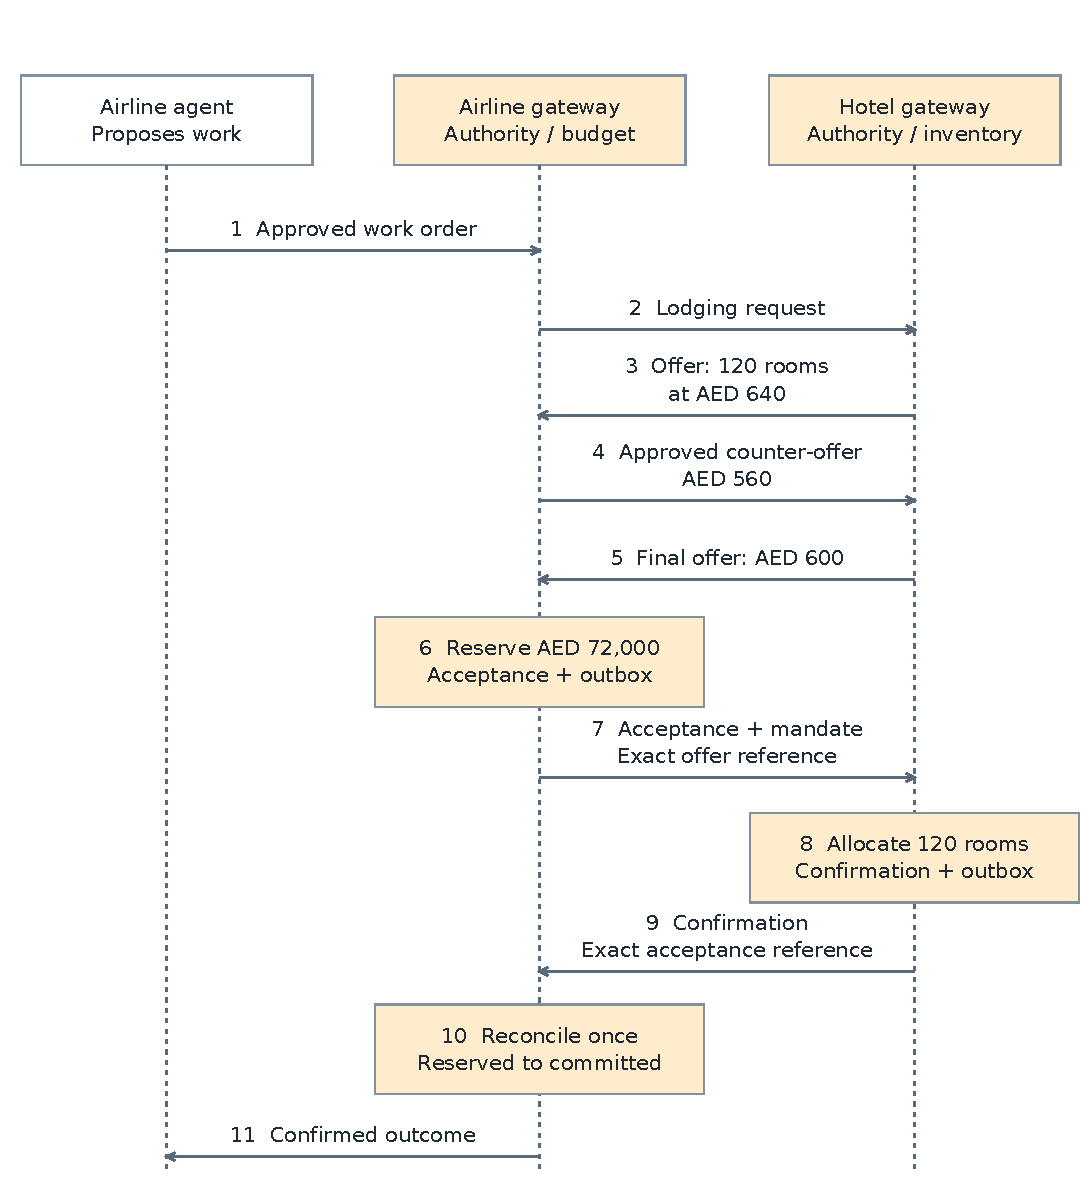
\includegraphics[width=\textwidth]{figures/booking-sequence.pdf}
\caption{Illustrative accommodation sequence for 120 rooms. Time runs down the participant lifelines. Gateway-to-gateway arrows denote logical exchanges through the restricted deal channel, not direct transport or immediate delivery. Local boxes show atomic ledger and durable-record updates: airline reservation precedes acceptance publication, and hotel allocation precedes confirmation publication. Reconciliation transfers reserved exposure to committed exposure once. The sequence is proposed, not an observed transaction.}
\label{fig:example-sequence}
\end{figure}

Before acceptance, the airline gateway authenticates the requesting agent, verifies its delegated authority and checks the aggregate budget condition in Eq.~\ref{eq:method-budget}. The AED~72,000 must remain available after accounting for existing commitments and reservations, including any bookings made with other hotels. In one local transaction, the gateway reserves that amount, stores acceptance of the exact final offer and records the mandate and publication-outbox entry. The mandate authorises this obligation for this counterparty without exposing the airline's total budget. A publication worker then sends the stored record to the deal PDS. The reservation therefore exists before the hotel necessarily sees the acceptance.

The hotel gateway verifies the acceptance's offer reference and authority evidence, checks that the revision remains undecided and within its decision deadline, and applies the inventory condition in Eq.~\ref{eq:method-stock}. If at least 120 suitable rooms remain allocatable, it records confirmation and allocates those rooms in one transaction. Otherwise, it records closure. Both outcomes use the same terminal decision slot, so closure and confirmation cannot both be admitted under the specified gateway rules. Confirmation establishes the protocol commitment defined in Eq.~\ref{eq:method-commit}; the framework agreement determines its contractual effect. Receipt of that confirmation converts the airline's reservation to committed exposure without increasing its total accounted exposure.

Figure~\ref{fig:example-reservation} isolates the airline's accounting from the message sequence. It follows an accepted deal and shows why a timeout preserves the reservation even when the hotel may already have confirmed. A delayed confirmation illustrates why the recovery rule matters. Suppose the hotel allocates the rooms and durably records confirmation, but the airline has not received it when the deadline passes. The airline cannot distinguish that situation from an undecided booking merely by observing silence. It therefore retains the AED~72,000 reservation and seeks the terminal record. Releasing the funds would allow the same budget to support another booking while the first obligation still exists. If the hotel instead records closure, the airline releases the reservation only after verifying that closure. Repeated delivery must not repeat either accounting operation. A crash after a local decision but before publication is handled by publishing the existing outbox entry, not by creating a second acceptance or allocating another 120 rooms.

\begin{figure}[htbp]
\centering
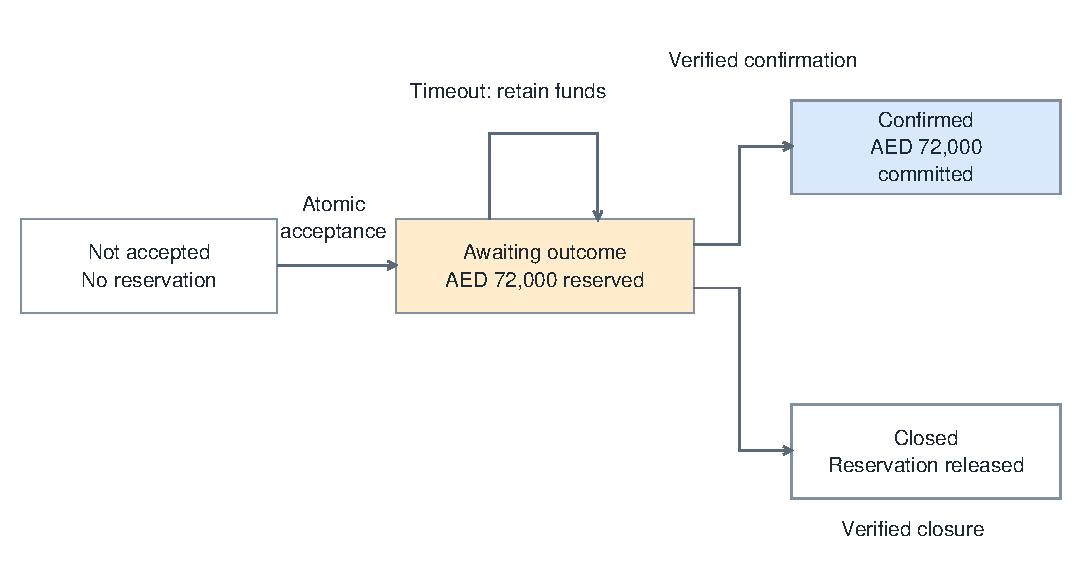
\includegraphics[width=\textwidth]{figures/booking-reservation-states.pdf}
\caption{Buyer accounting for the illustrative 120-room deal. Acceptance reserves AED~72,000. Verified confirmation transfers that amount to committed exposure; verified closure releases it. A timeout returns to the awaiting-outcome state because confirmation may exist before its evidence arrives. Reconciliation applies each terminal outcome once. The figure follows the normal acceptance path; closure received before acceptance instead records a closed revision and prevents later acceptance, as specified in Algorithm~\ref{alg:method-admission}.}
\label{fig:example-reservation}
\end{figure}

After confirmation, an authorised A2A task may transfer the necessary rooming information through an approved execution channel. The operation identifier contains the deal, revision and action, allowing the receiving business system to suppress duplicate execution or reconcile an uncertain response. Passenger information is released only if a separate approved work order permits it. An invoice later refers to the confirmed terms and performance evidence; settlement remains a separate event and does not redefine when the booking became committed. Replacement bookings and amendment accounting are outside this initial-commitment walkthrough.

The example shows how the method connects conversation to business state. Linked records identify the final terms and the decisions leading to them. The mandate identifies the permitted action, while the airline and hotel ledgers determine whether that action has financial and inventory backing. The release interface limits what each outbound message contains, and retained terminal evidence supports recovery when publication or delivery is interrupted. These are the specified responsibilities of the proposed method; the example does not establish their effectiveness in a running multi-organisation deployment.
